%-------------------------------------------------------------------------------
\section{Truth-level \texorpdfstring{$p_{T}$}{pt} and \texorpdfstring{$\eta$}{eta} distributions of Signal MC samples}
\label{app:signal_truth}
%-------------------------------------------------------------------------------
The representative plots of truth-level $p_{T}$ and $\eta$ distributions of $Z'$ and the muons from the decay of $Z'$, referred as \textit{signal} muons, are shown in Figure~\ref{fig:truth_zp_muon} using the signal MC samples with $m=$ 500, 1000 GeV and $c\tau=$ 100 mm. The signal MC samples with $ee$ and $e\mu$ final states produce similar distributions.

The $\eta$ distribution of signal muons shows that most of the signal muons are produced within the detector acceptance ($\eta <$ 2.7). The characteristic upper edge in the $p_{T}$ spectrum is related to the $Z'$ mass.


\begin{figure}[!htb]
    \centering
    \subfloat[]{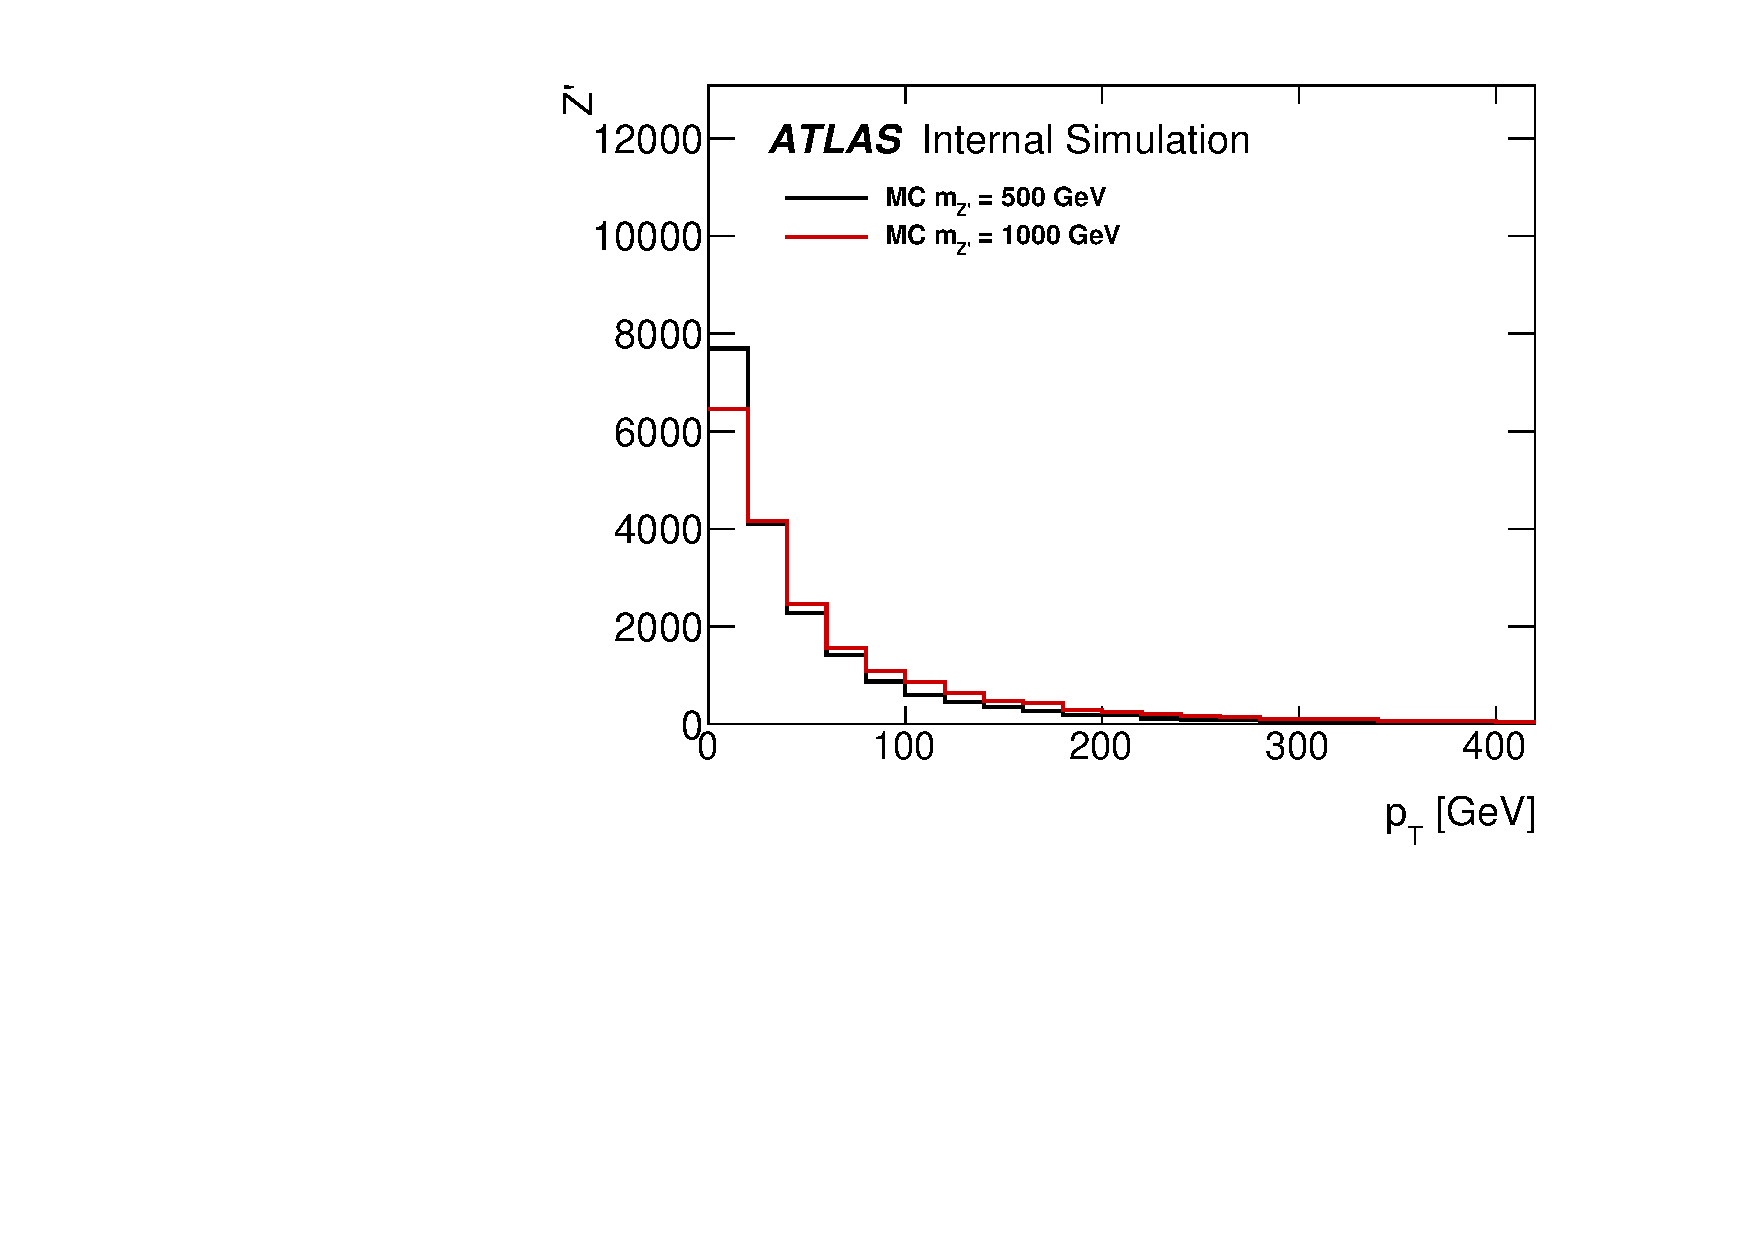
\includegraphics[width=0.45\textwidth]{figures/m_truth_zp_pt.pdf}}
    \subfloat[]{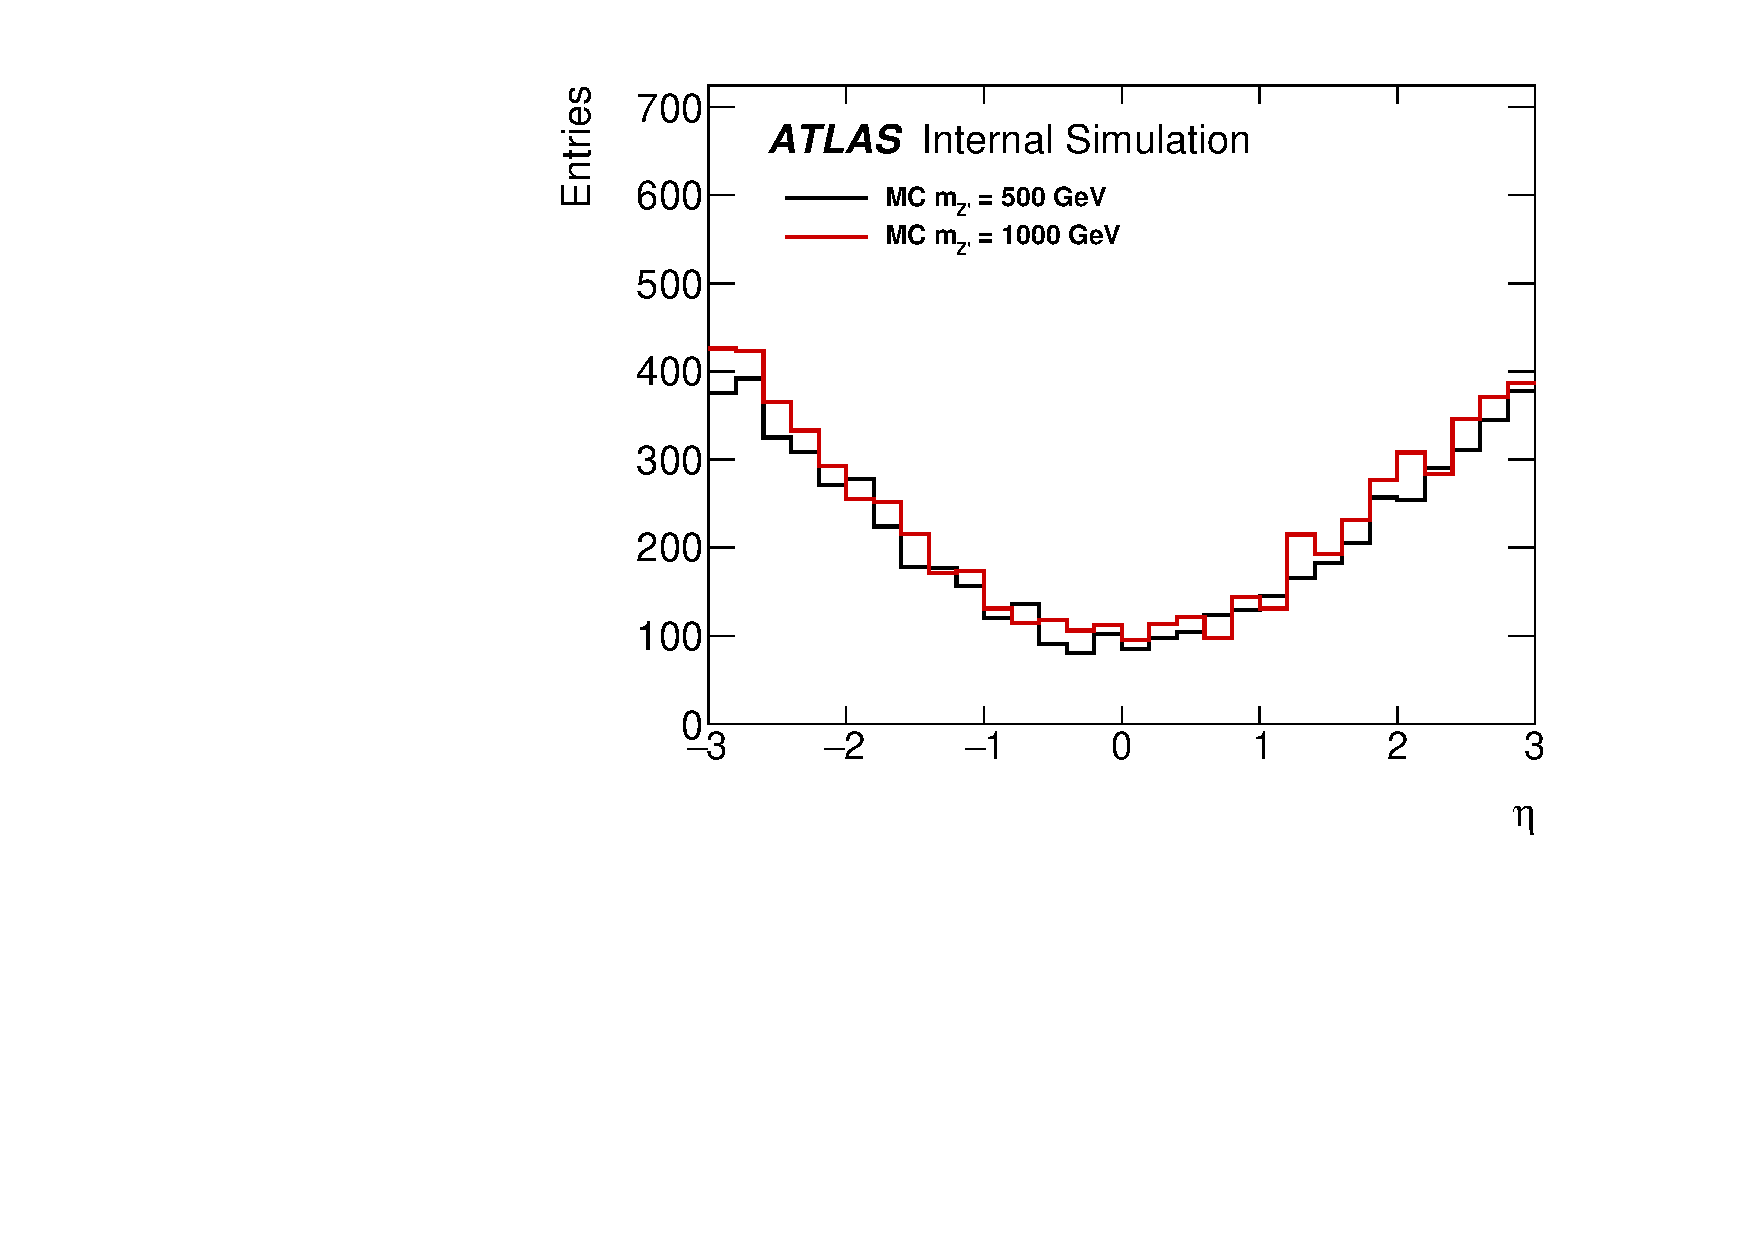
\includegraphics[width=0.45\textwidth]{figures/m_truth_zp_eta.pdf}} \\
    \subfloat[]{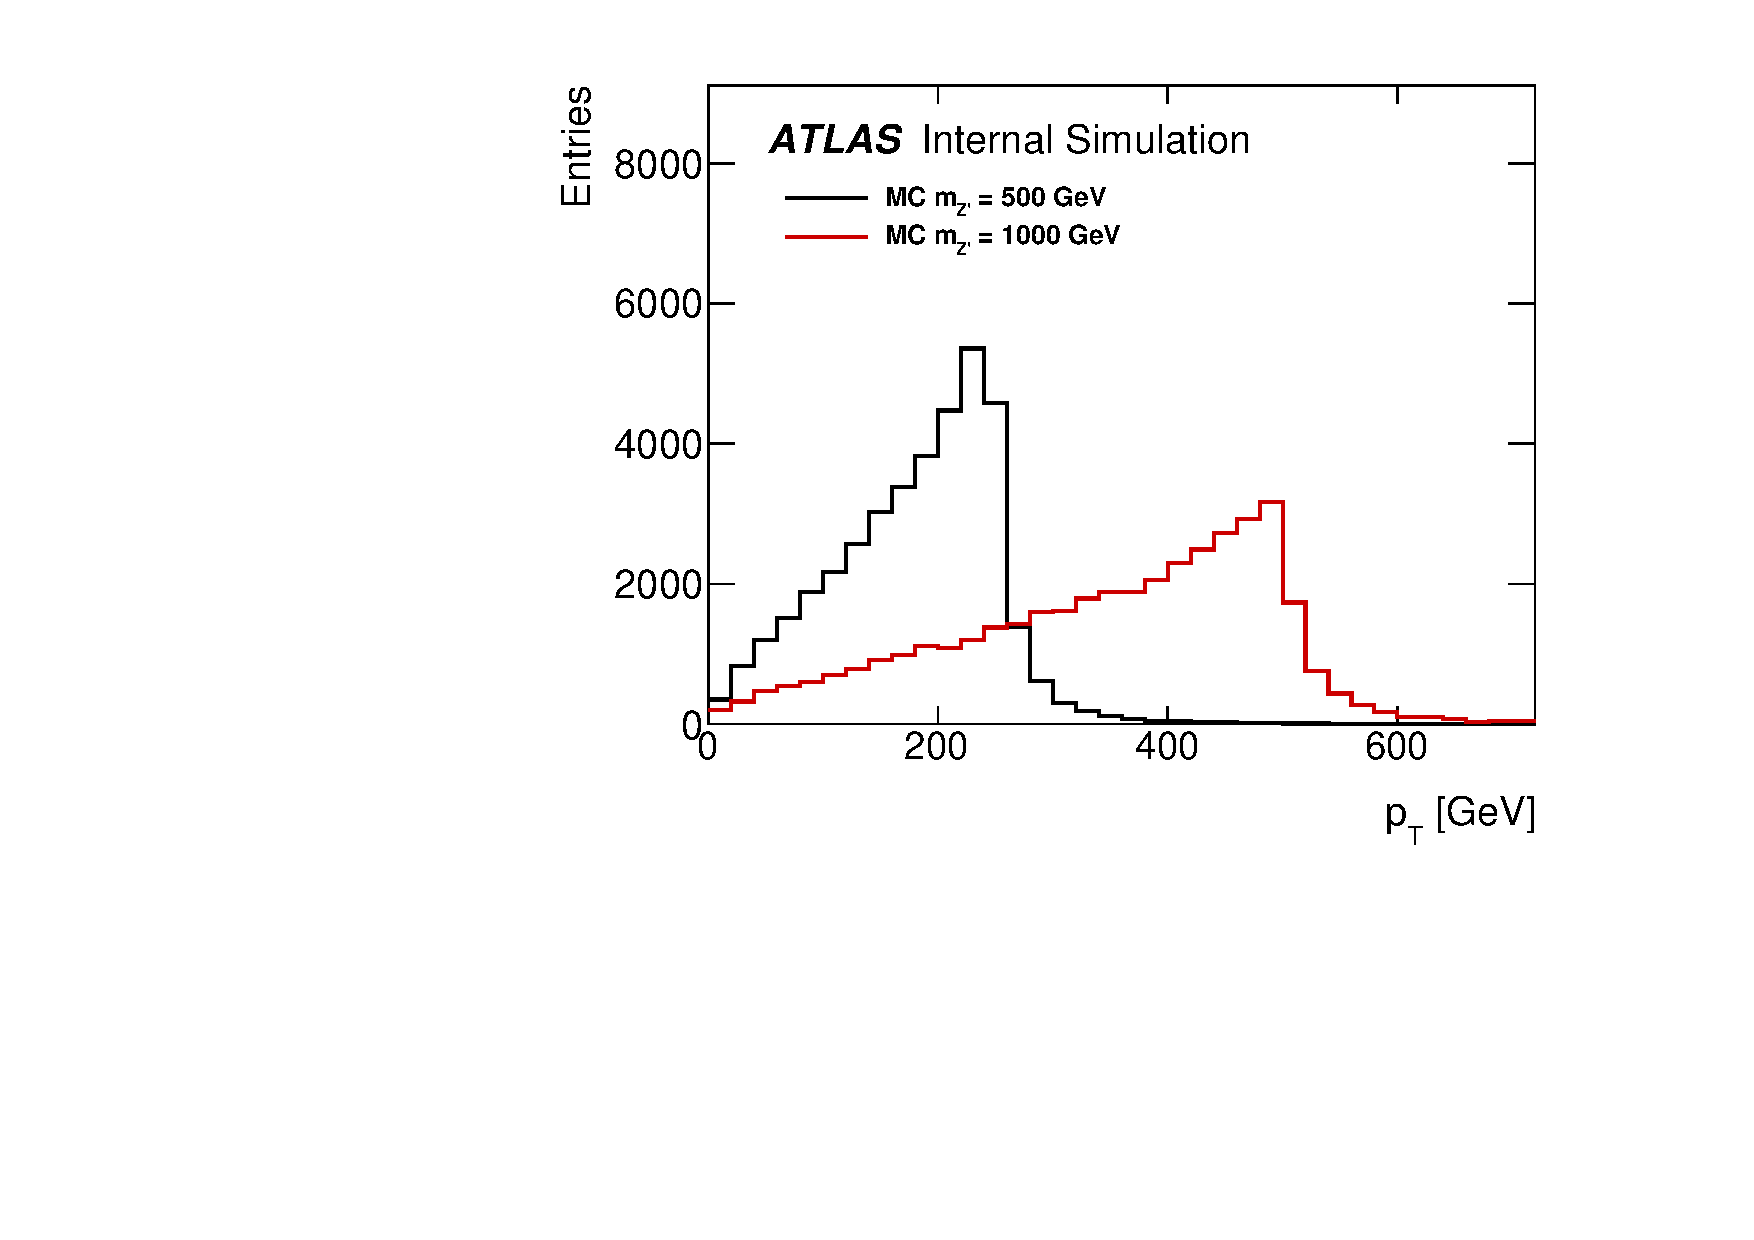
\includegraphics[width=0.45\textwidth]{figures/m_truth_muon_pt.pdf}}
    \subfloat[]{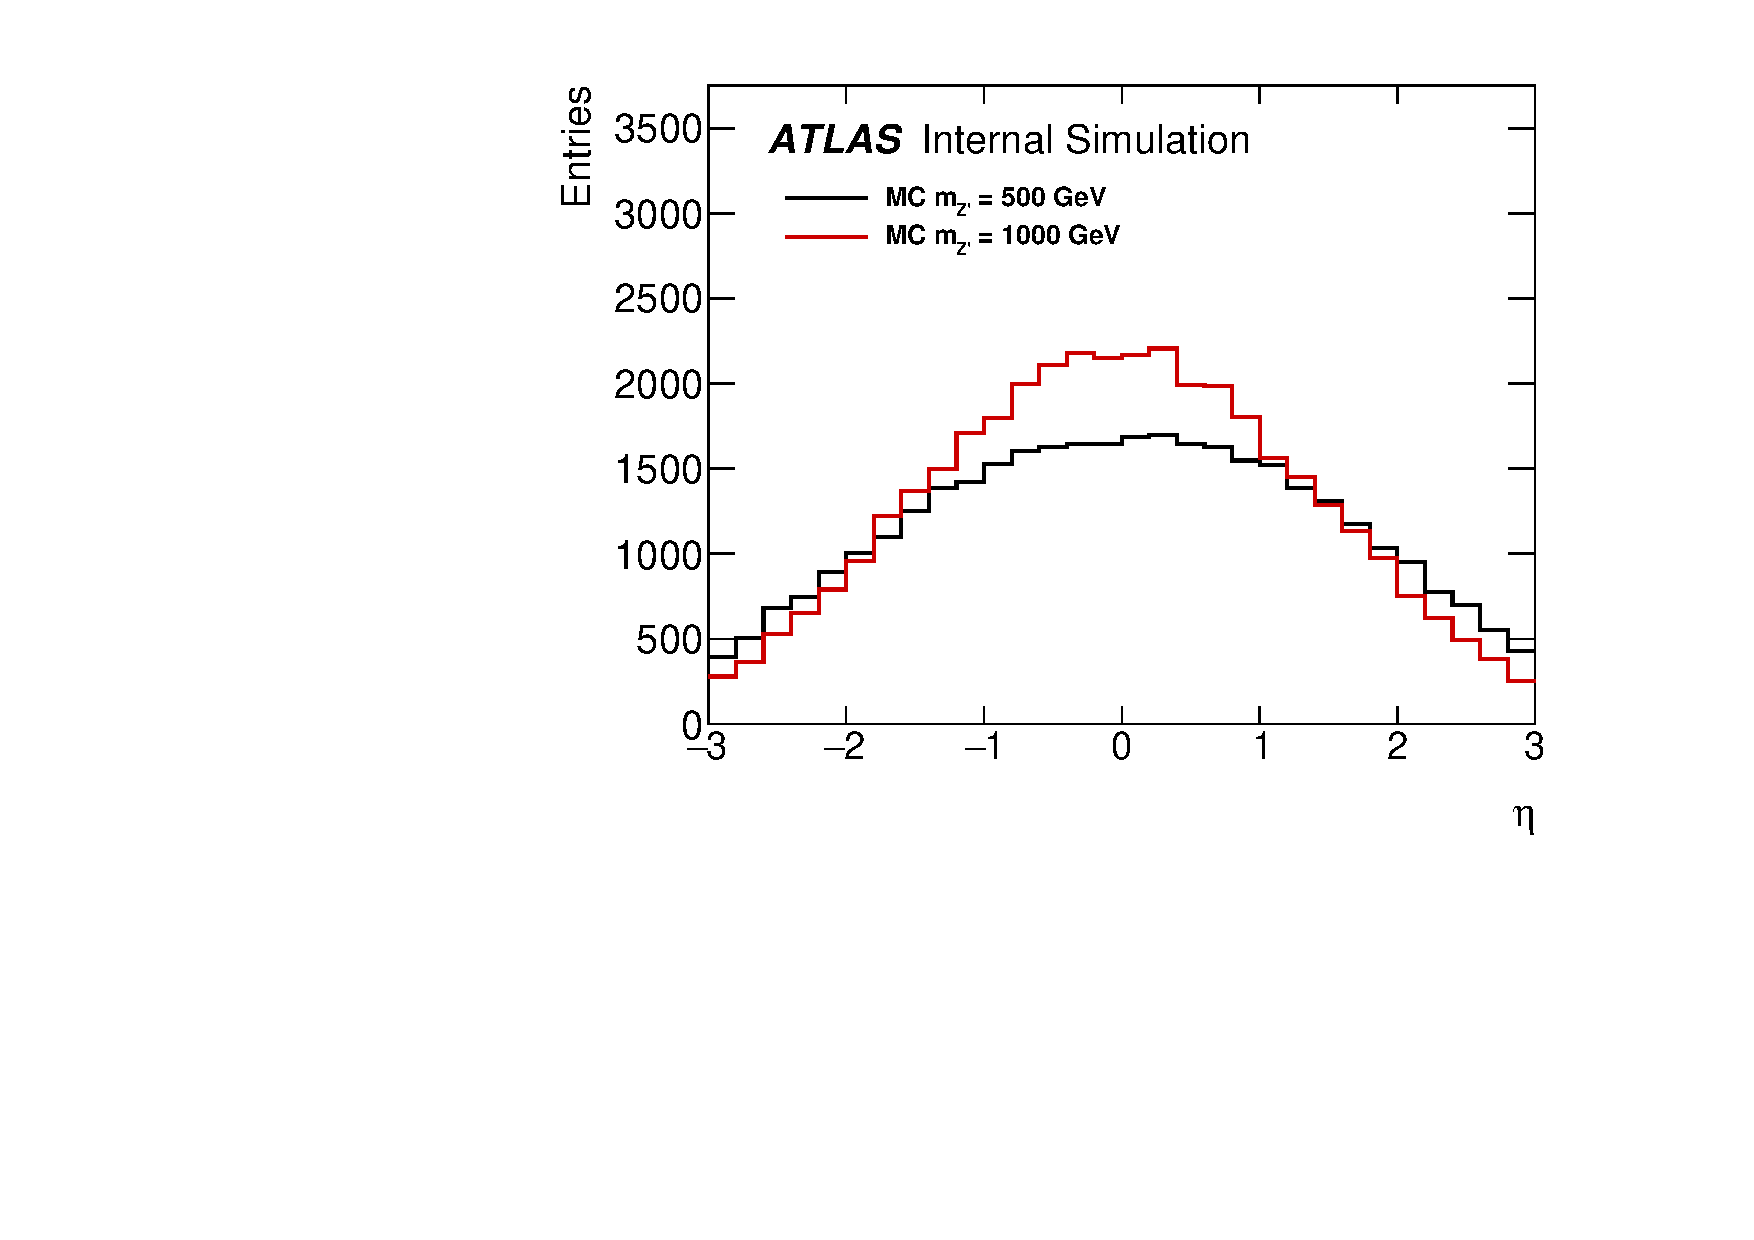
\includegraphics[width=0.45\textwidth]{figures/m_truth_muon_eta.pdf}}
    \caption{The representative plots of truth-level (a) $p_{T}$ and (b) $\eta$ distributions of $Z'$, and (c), (d) are the corresponding distributions for the signal muons. The signal MC samples are generated with $m=$ 500, 1000 GeV, and $c\tau=$ 100 mm.}
    \label{fig:truth_zp_muon}
\end{figure}
